\chapter{短波语音主观评价在线辅助系统} \label{chapter:web}


客观评分算法的目标是希望能够尽量逼近人的主观感受,为了验证本文客观评分算法的效果,需要获得短波语音的主观平均意见分,即MOS(Mean Opinion Score)。由于低信噪比的短波信道语音质量相对较低,且浮动范围大,志愿者在不知道语音整体质量范围的情况下直接打分,结果会有失偏颇。所以本文先对随机选取的短波语音按照主观比较结果进行排序,确定短波语音的整体质量范围,从而确定评分的参考标准。
为方便短波语音的主观排序和MOS分生成,本文实现了一个在线辅助系统,志愿者可以在线试听、比较、评价短波语音,可用于组织短波语音的主观评价实验。

\section{系统功能介绍}

短波语音主观评价辅助系统主要具有两大功能,一是通过和志愿者的交互,对一系列短波语音按照主观感受质量进行排序;二是通过搜集志愿者对短波语音的评分,计算各个短波语音的平均主观意见分。

\begin{figure}
\centering
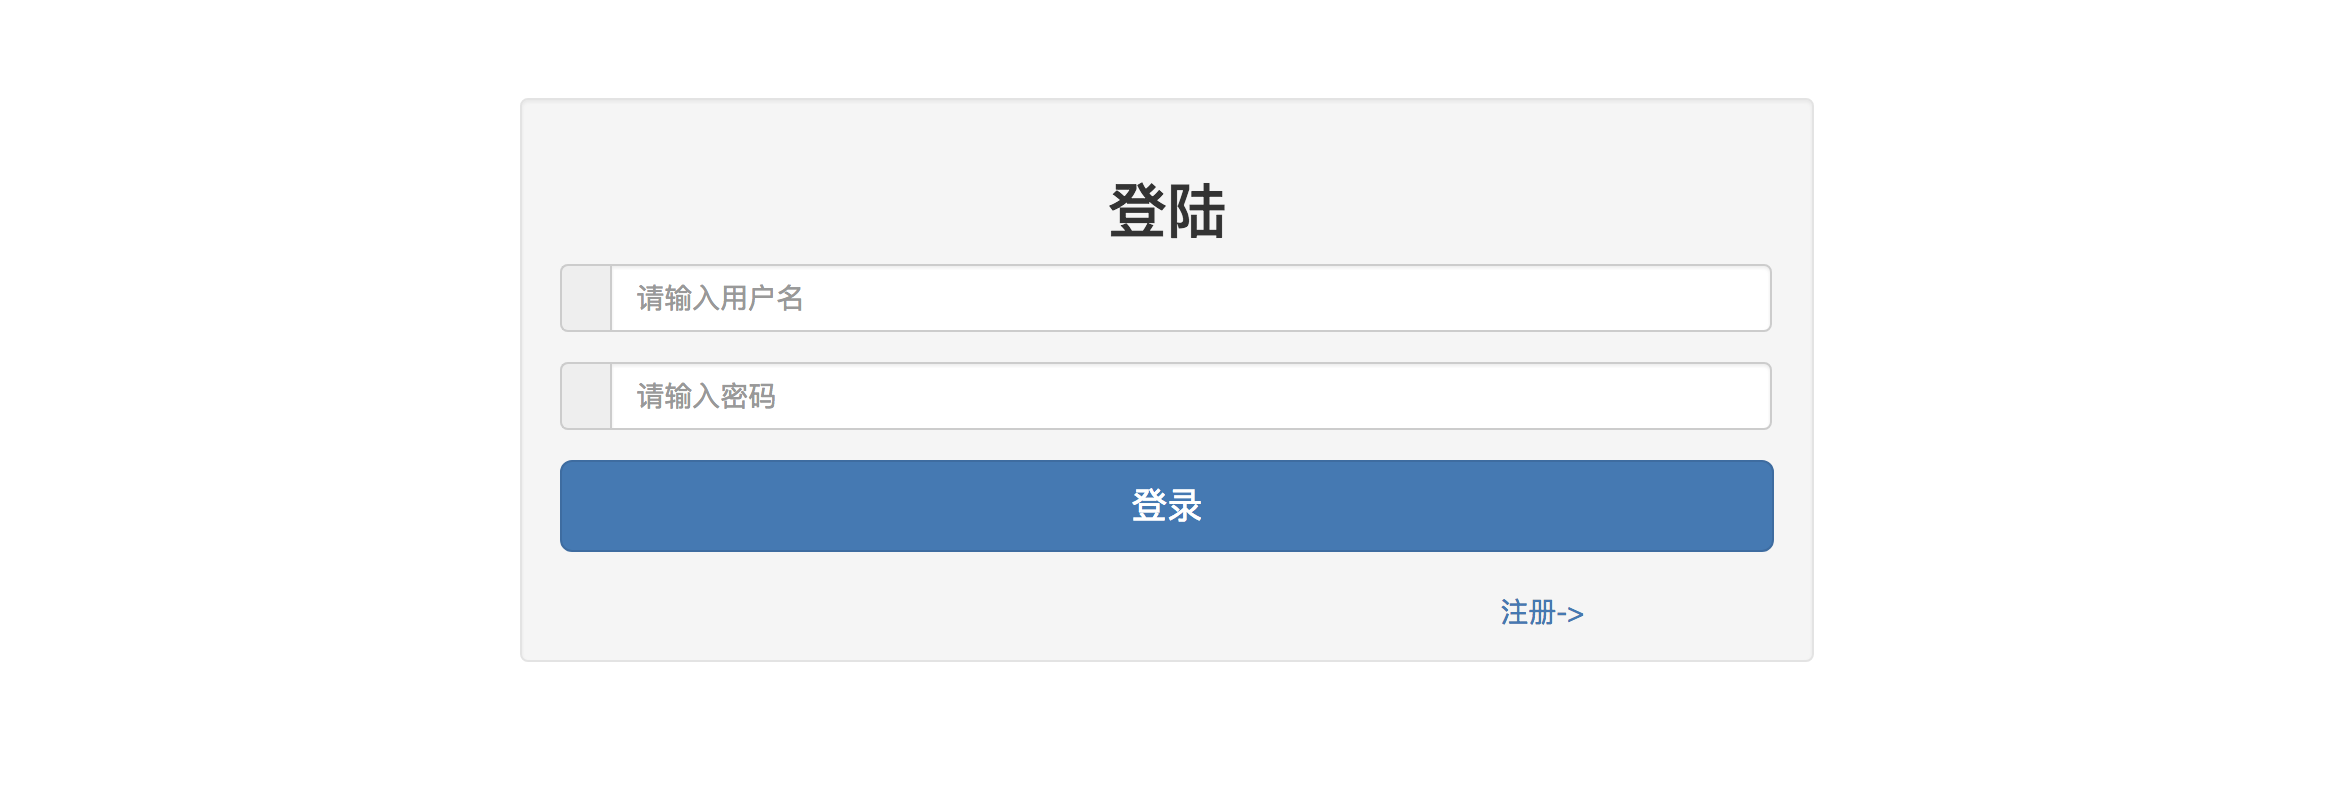
\includegraphics[width=0.8\textwidth]{web-login}
\caption{在线辅助系统的登陆界面\label{fig:web-login}}
\end{figure}

该辅助系统分为管理端和志愿者端,如图~\ref{fig:web-login}为系统登录界面,使用管理员账户登录可进入管理端,否则进入志愿者端。点击“注册”可以进行志愿者账号注册。

\begin{figure}
\centering
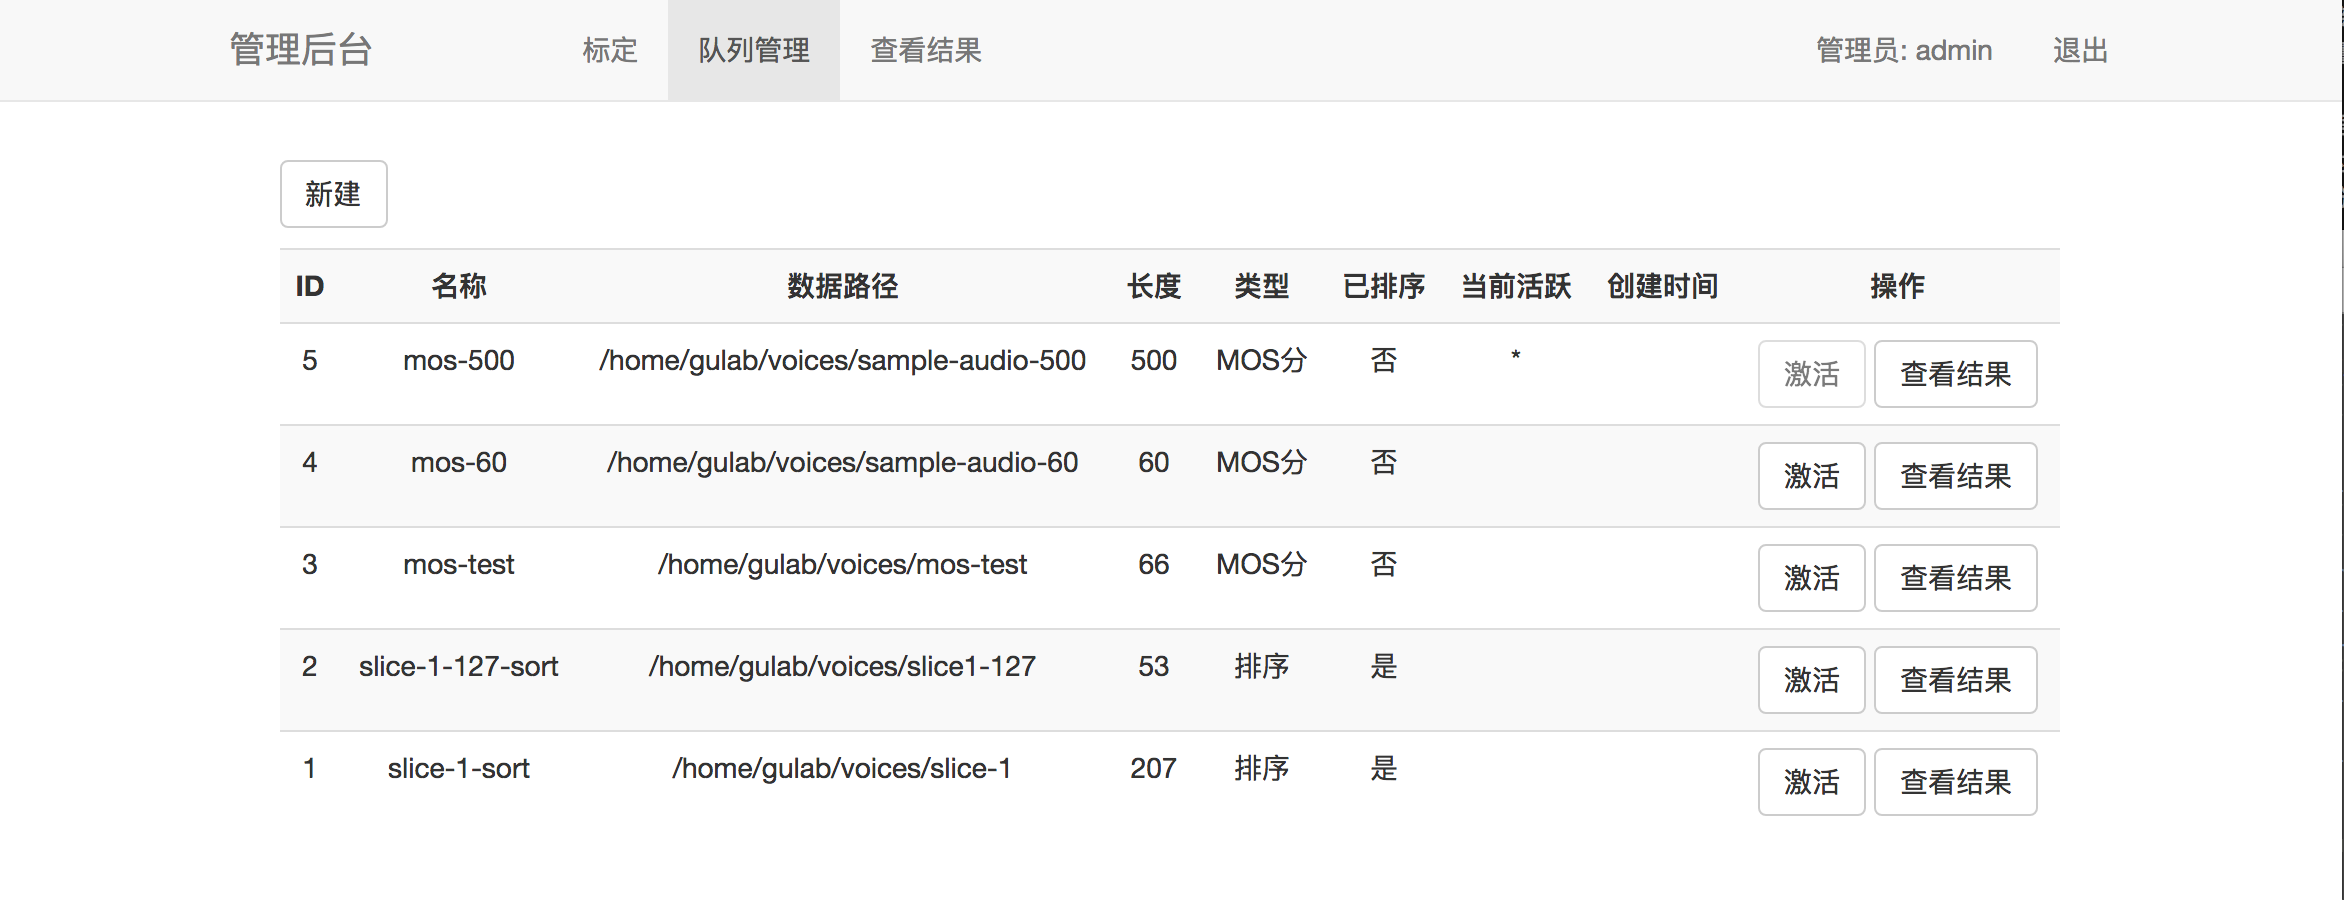
\includegraphics[width=0.8\textwidth]{web-queues}
\caption{在线辅助系统的队列管理界面\label{fig:web-queues}}
\end{figure}

\begin{figure}
\centering
\subcaptionbox{排序结果\label{fig:web-sort}}{
    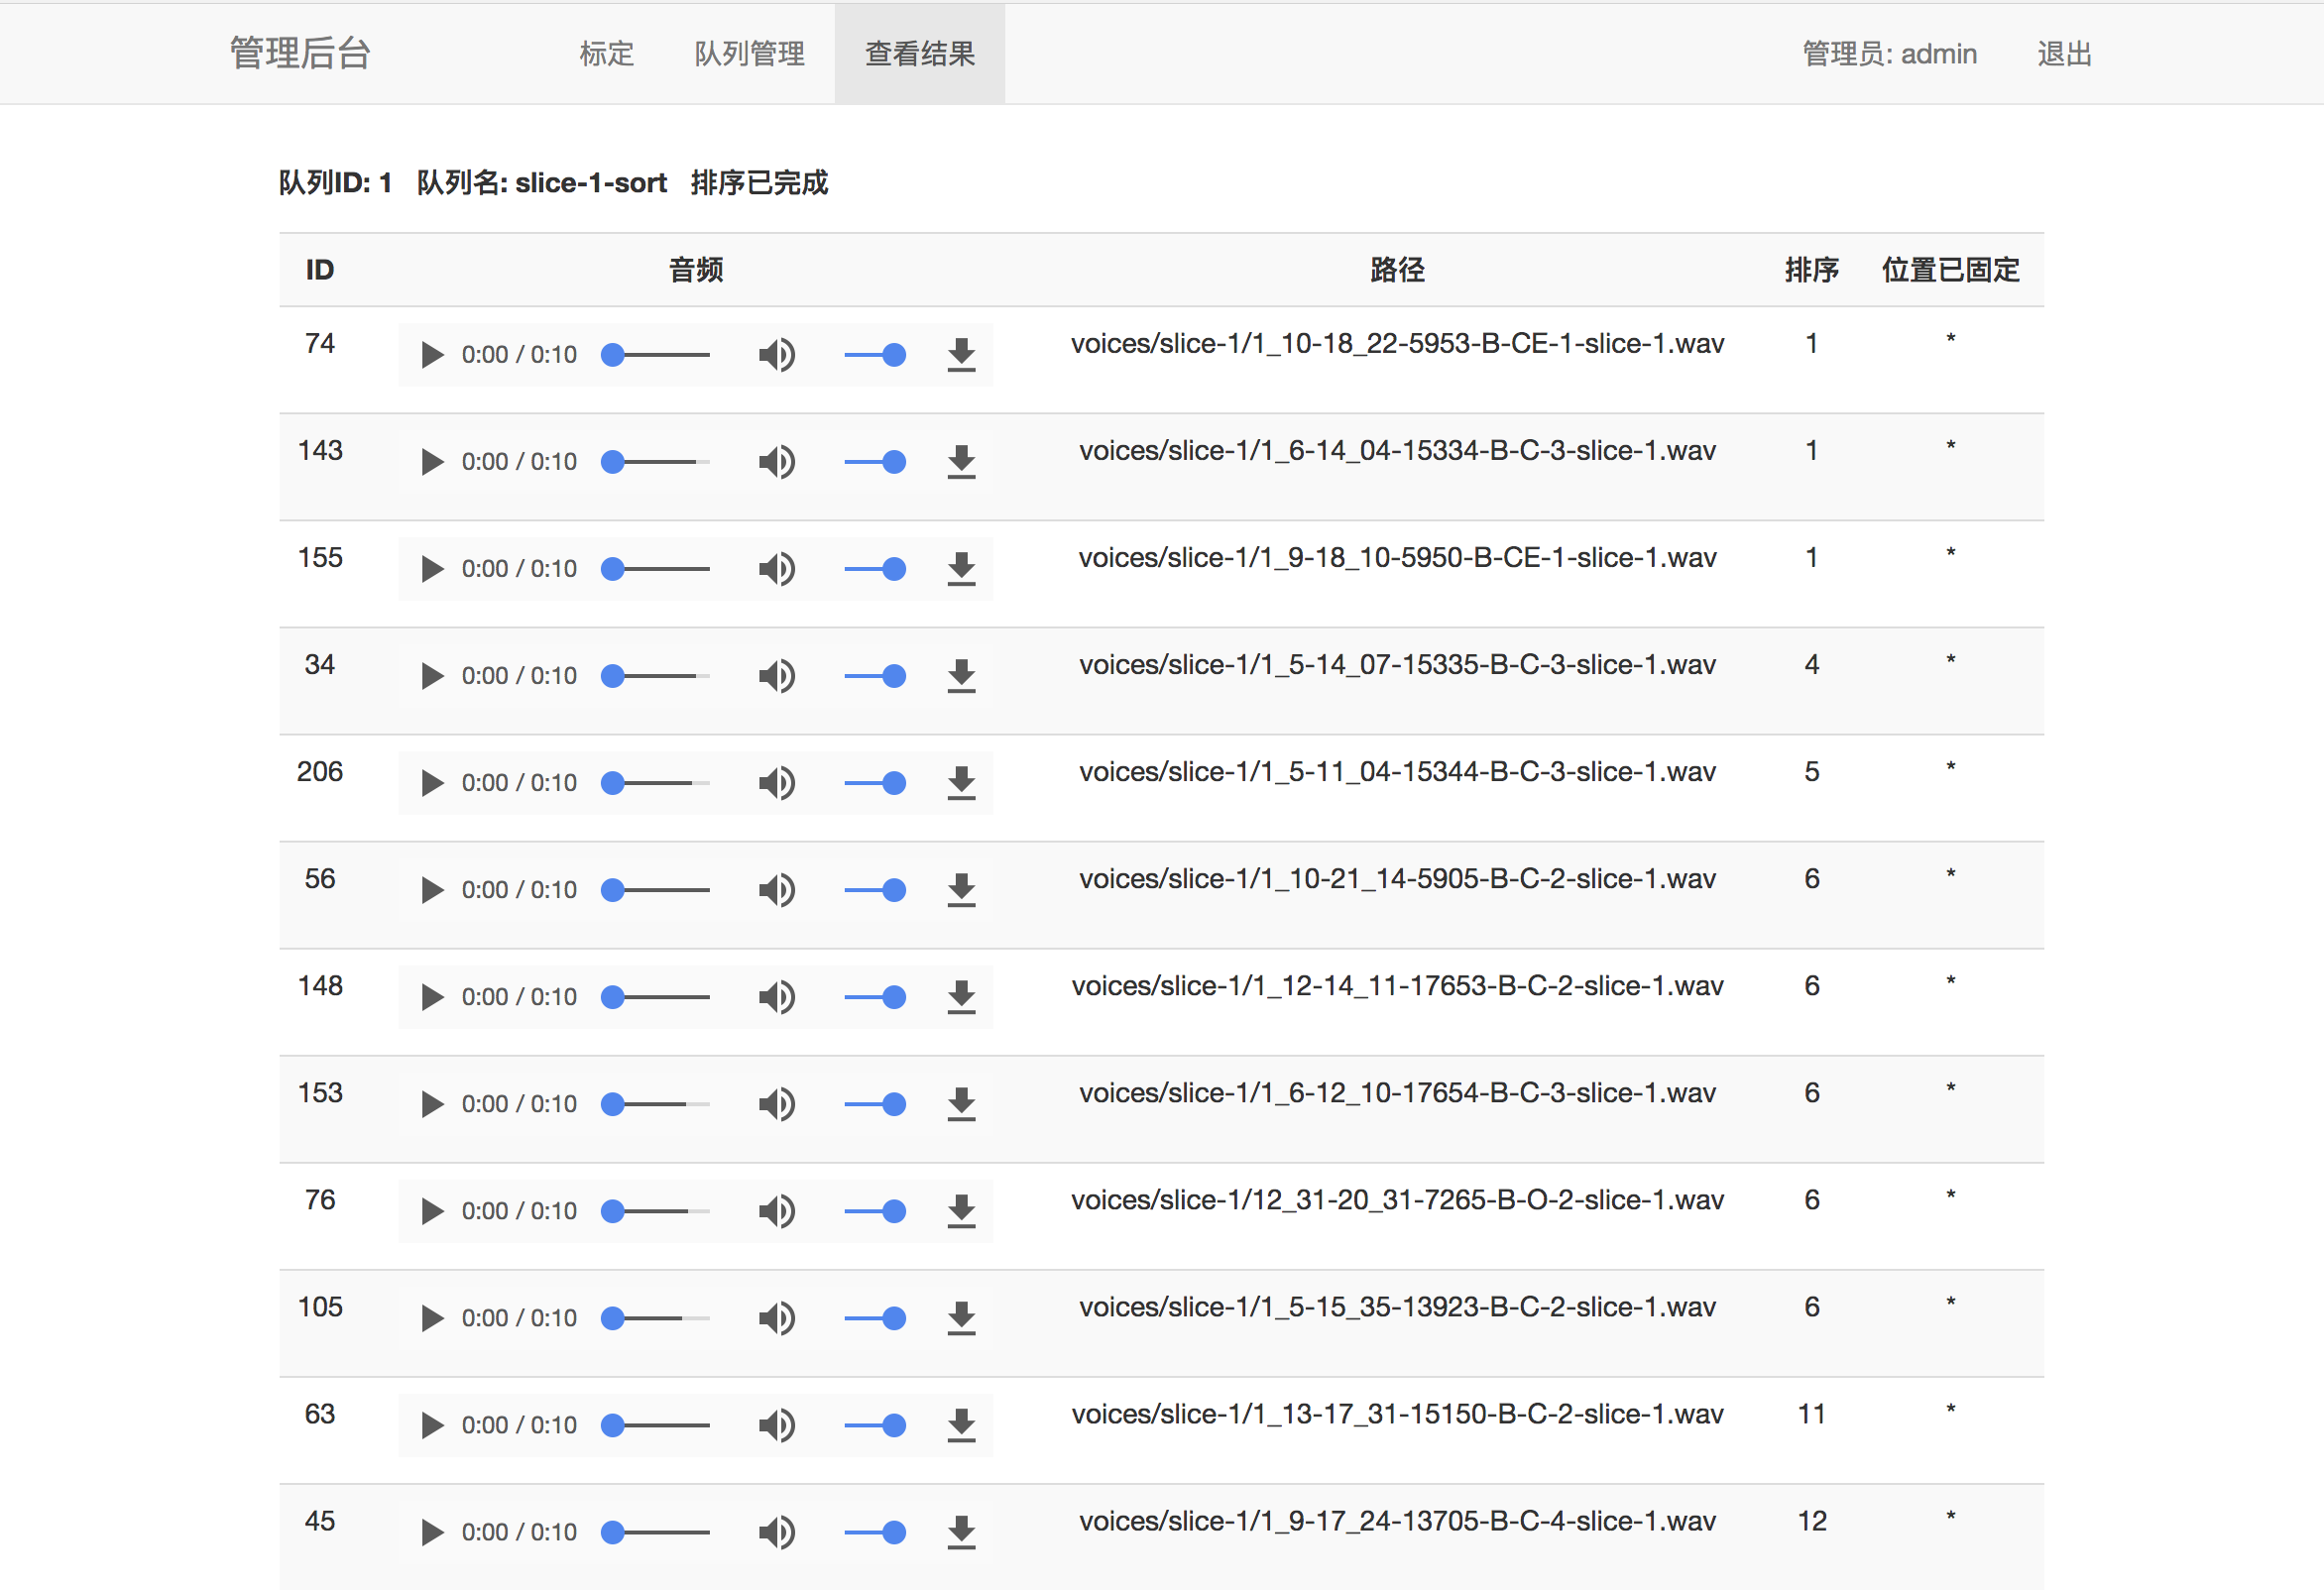
\includegraphics[width=0.45\textwidth]{web-sort}
}
\subcaptionbox{MOS分结果\label{fig:web-mos}}{
    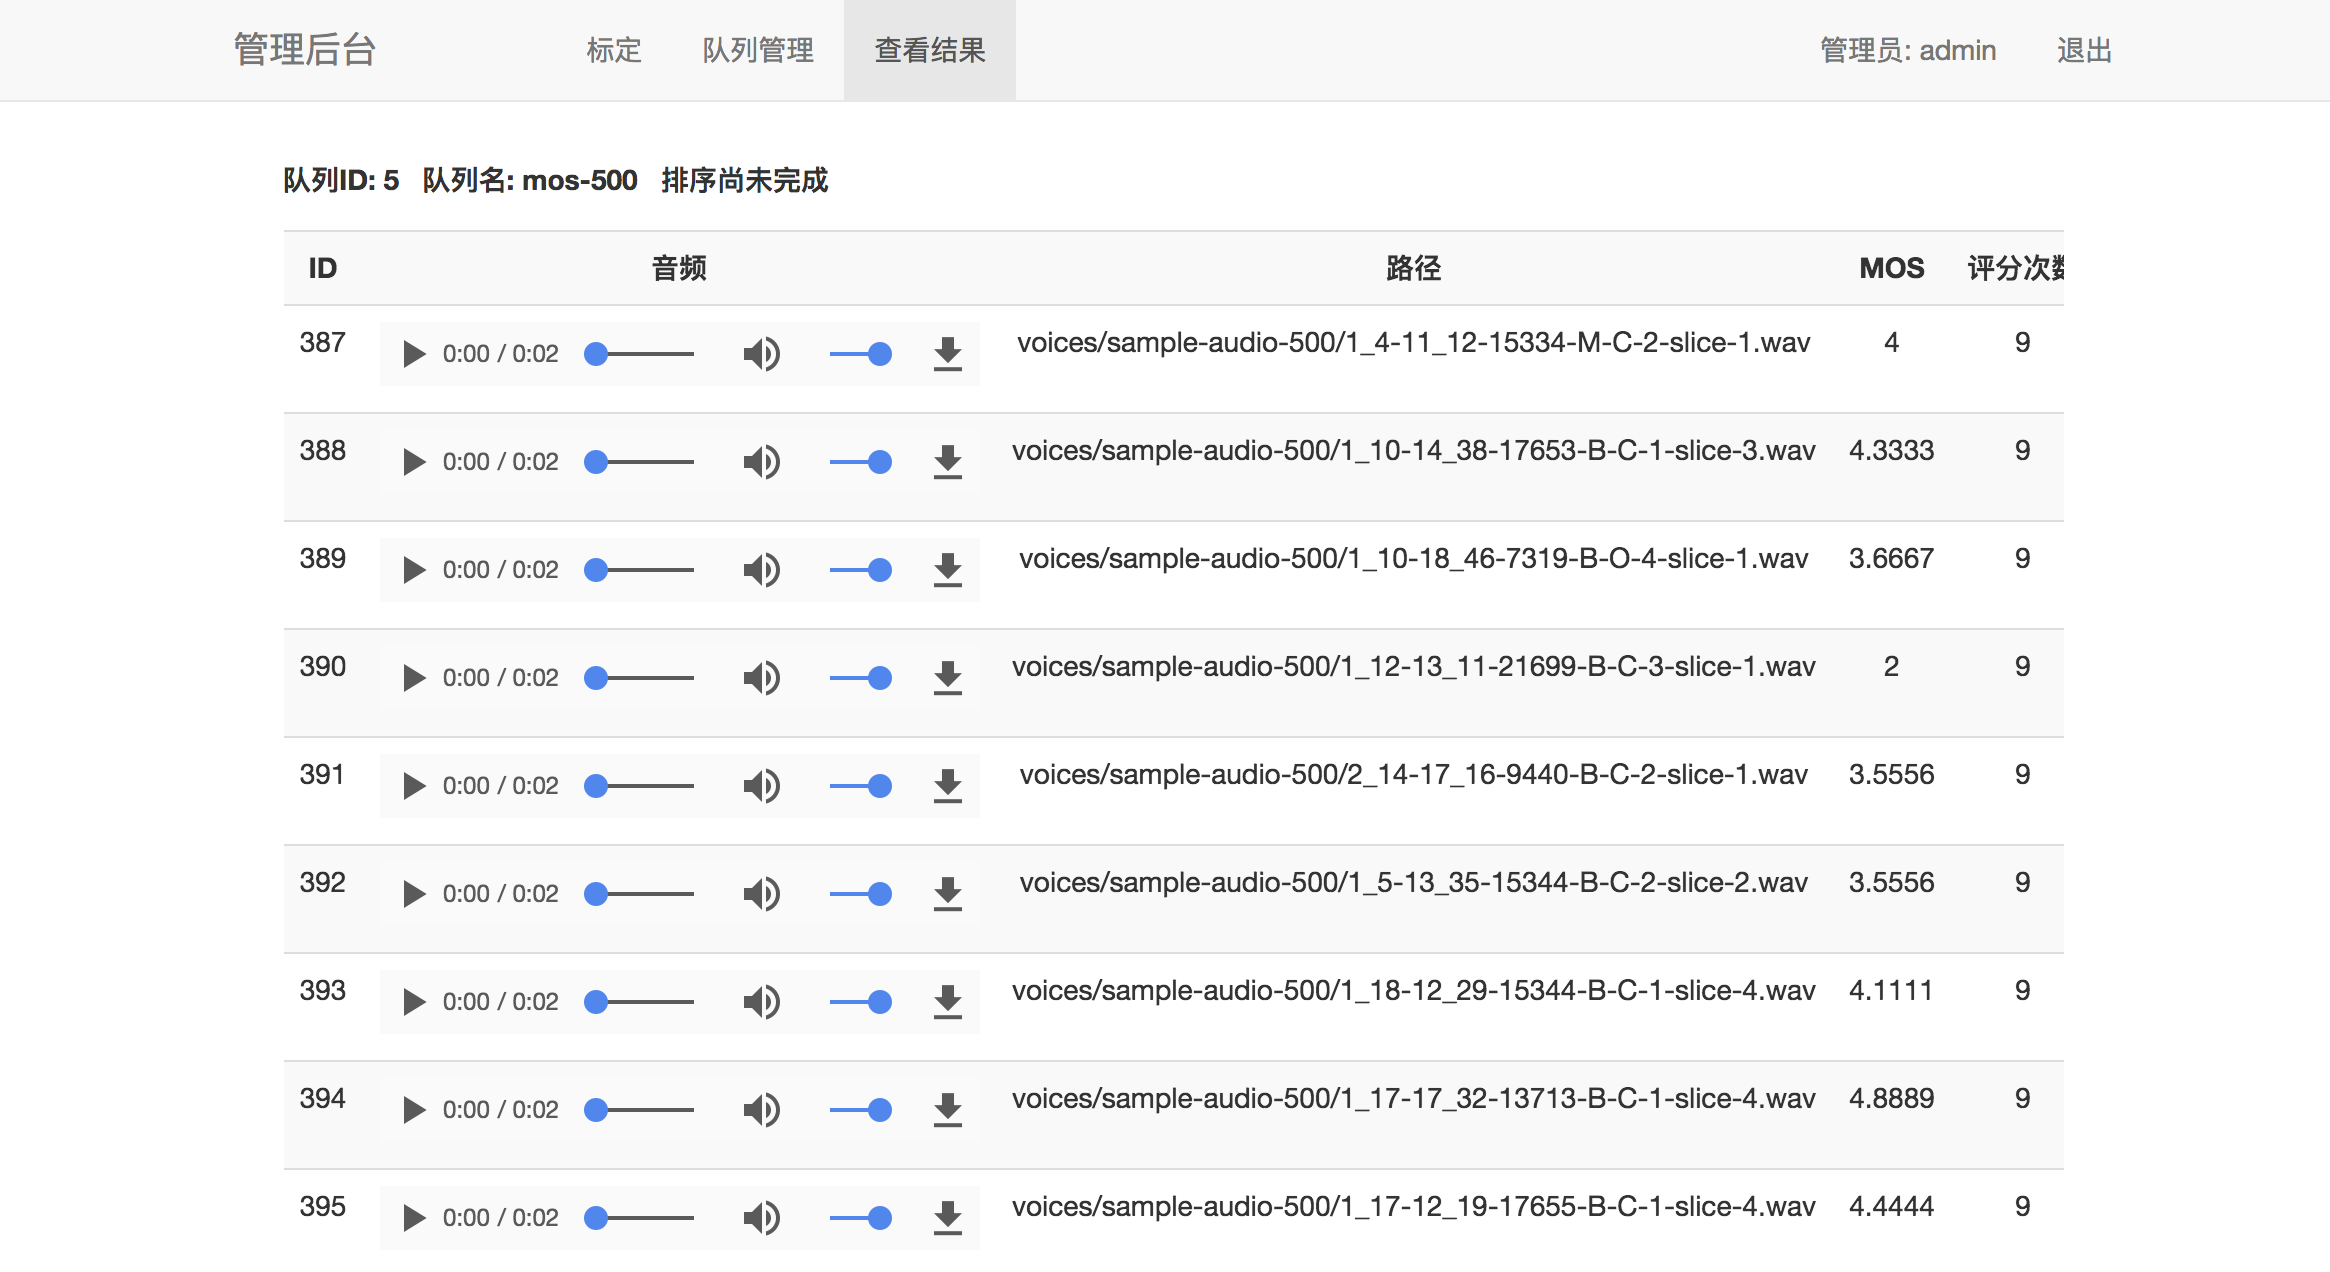
\includegraphics[width=0.45\textwidth]{web-mos}
}
\caption{在线辅助系统的队列结果界面\label{fig:web-result}}
\end{figure}

\begin{figure}
\centering
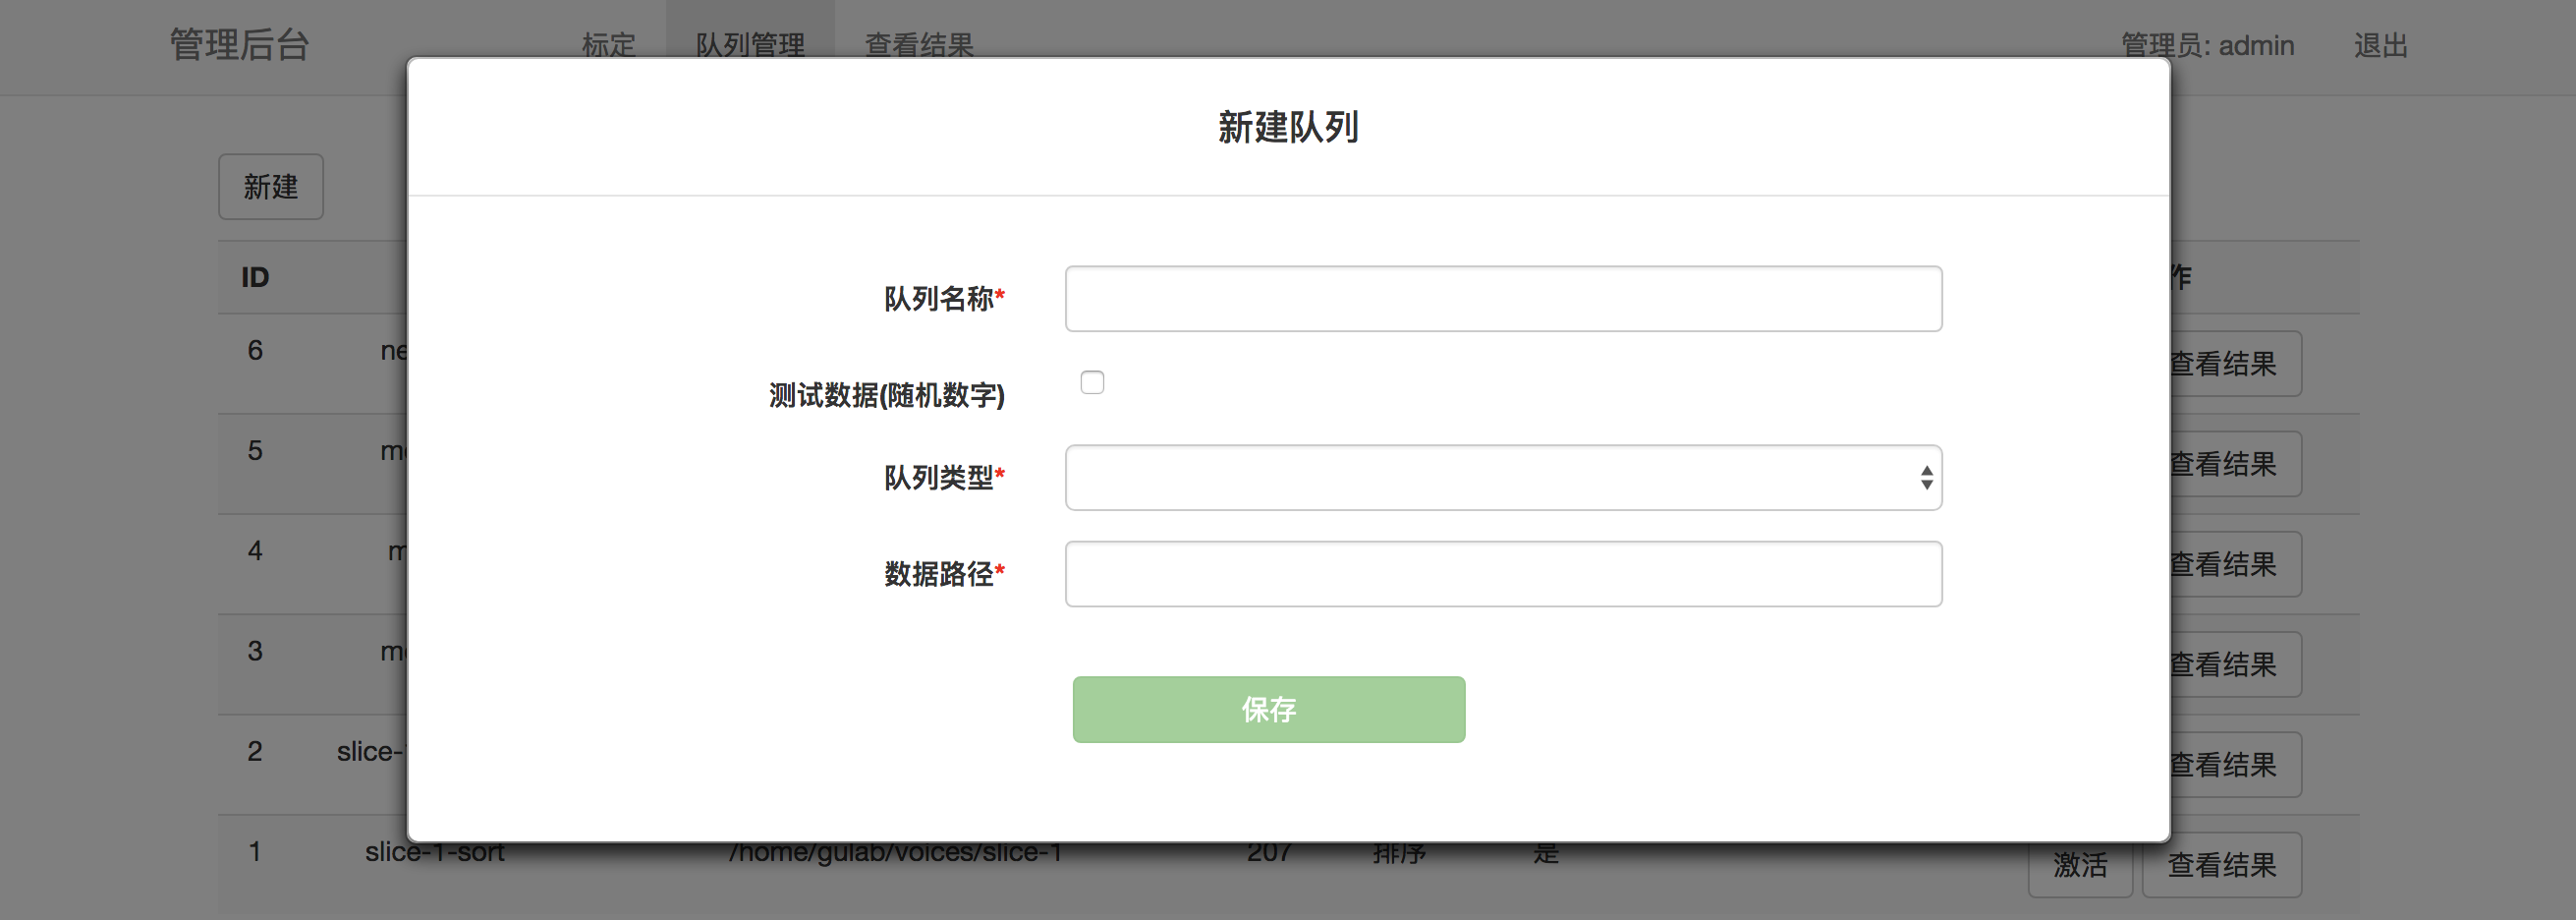
\includegraphics[width=0.8\textwidth]{web-new-queue}
\caption{在线辅助系统的新建队列界面\label{fig:web-new-queue}}
\end{figure}

管理端可以查看所有进行中和过往的主观评价实验,如图~\ref{fig:web-queues}所示,一次主观评价实验包含一系列短波语音,称为一个“语音队列”。队列类型有两种:“排序”、“MOS分”,分别对应于系统的两种功能。当前活跃的队列为正在进行的实验,志愿者看到的问题来自于该实验。可以点击”激活“来切换活跃的队列,点击”查看结果“来查看某一次实验的结果。点击“新建”按钮可以新建一个主观评价实验的语音队列。
图~\ref{fig:web-sort}为某一排序实验的结果,“排序”一列显示的是该语音在此队列中排序的位置,可以存在并列的情况。图~\ref{fig:web-mos}为某一MOS分实验结果,“MOS”一列表示当前计算的语音的MOS分,而“评分次数”表示当前完成对该语音的评分的志愿者数量。以上结果均可使用脚本进行导出,方便进一步基于主观评价结果的研究和实验。
图~\ref{fig:web-new-queue}为新建队列的界面,输入语音队列的名称,数据路径,选择实验类型,即可新建队列。系统后台会自动扫描数据路径下的语音数据,在系统中新建实验队列。

\begin{figure}
\centering
\subcaptionbox{排序任务\label{fig:web-user-sort}}{
    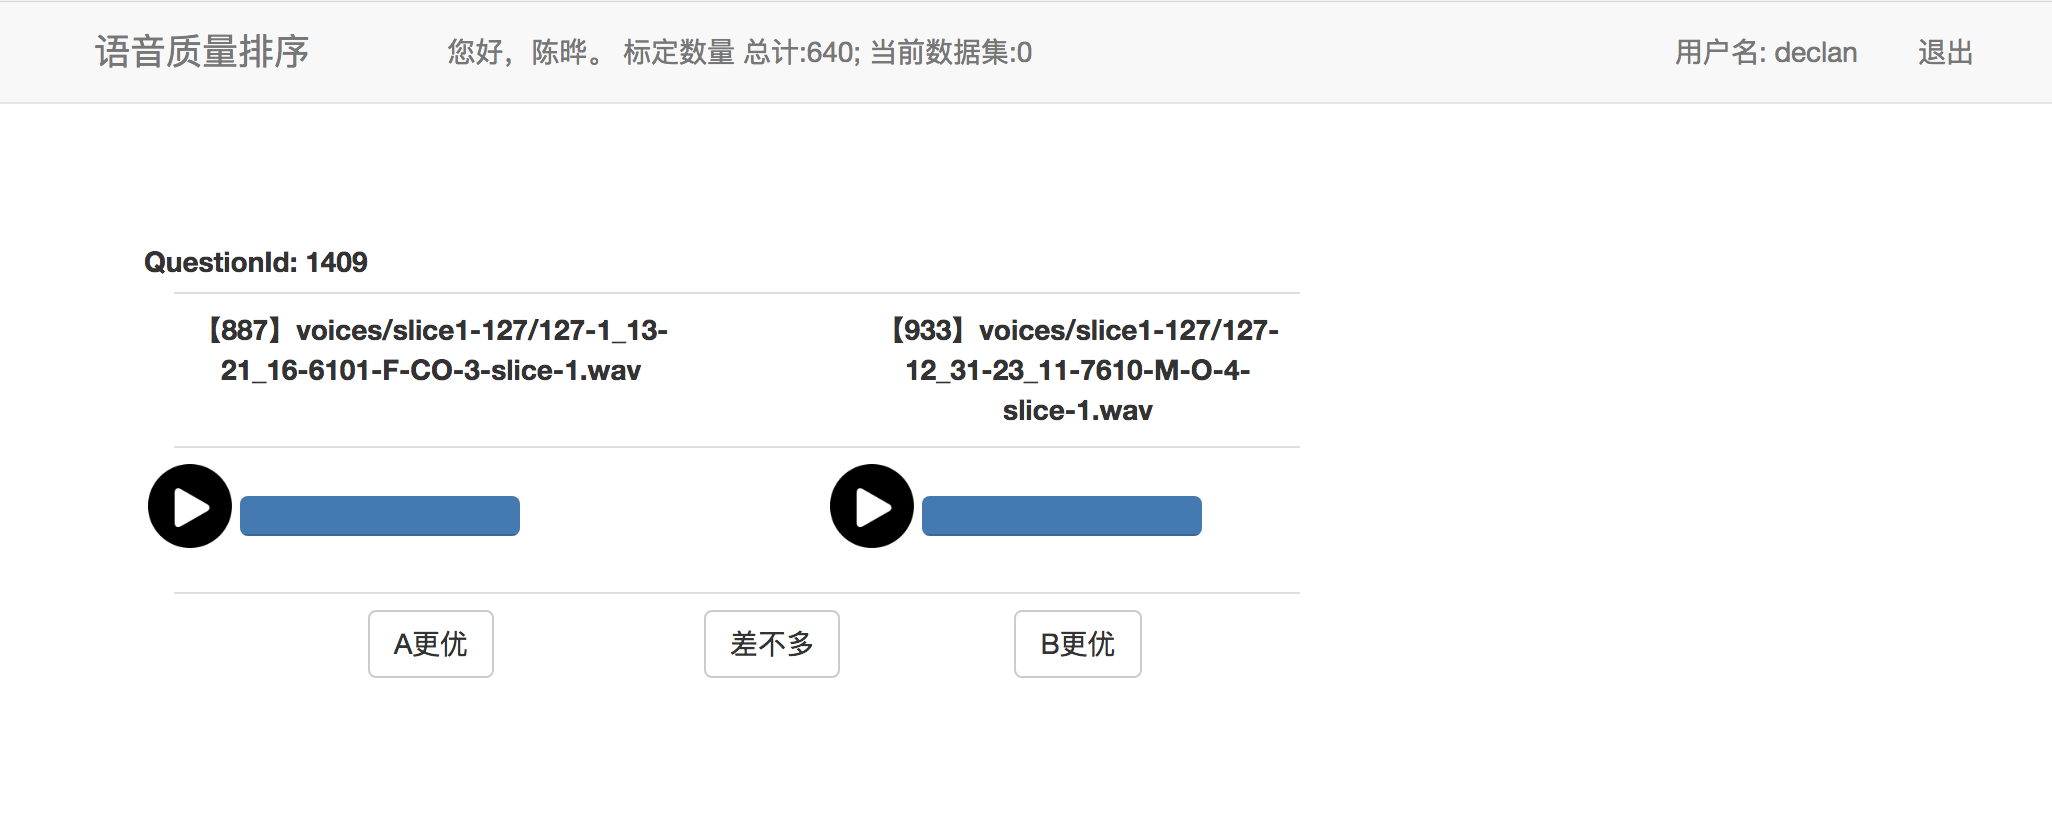
\includegraphics[width=0.45\textwidth]{web-user-sort}
}
\subcaptionbox{MOS分任务\label{fig:web-user-mos}}{
    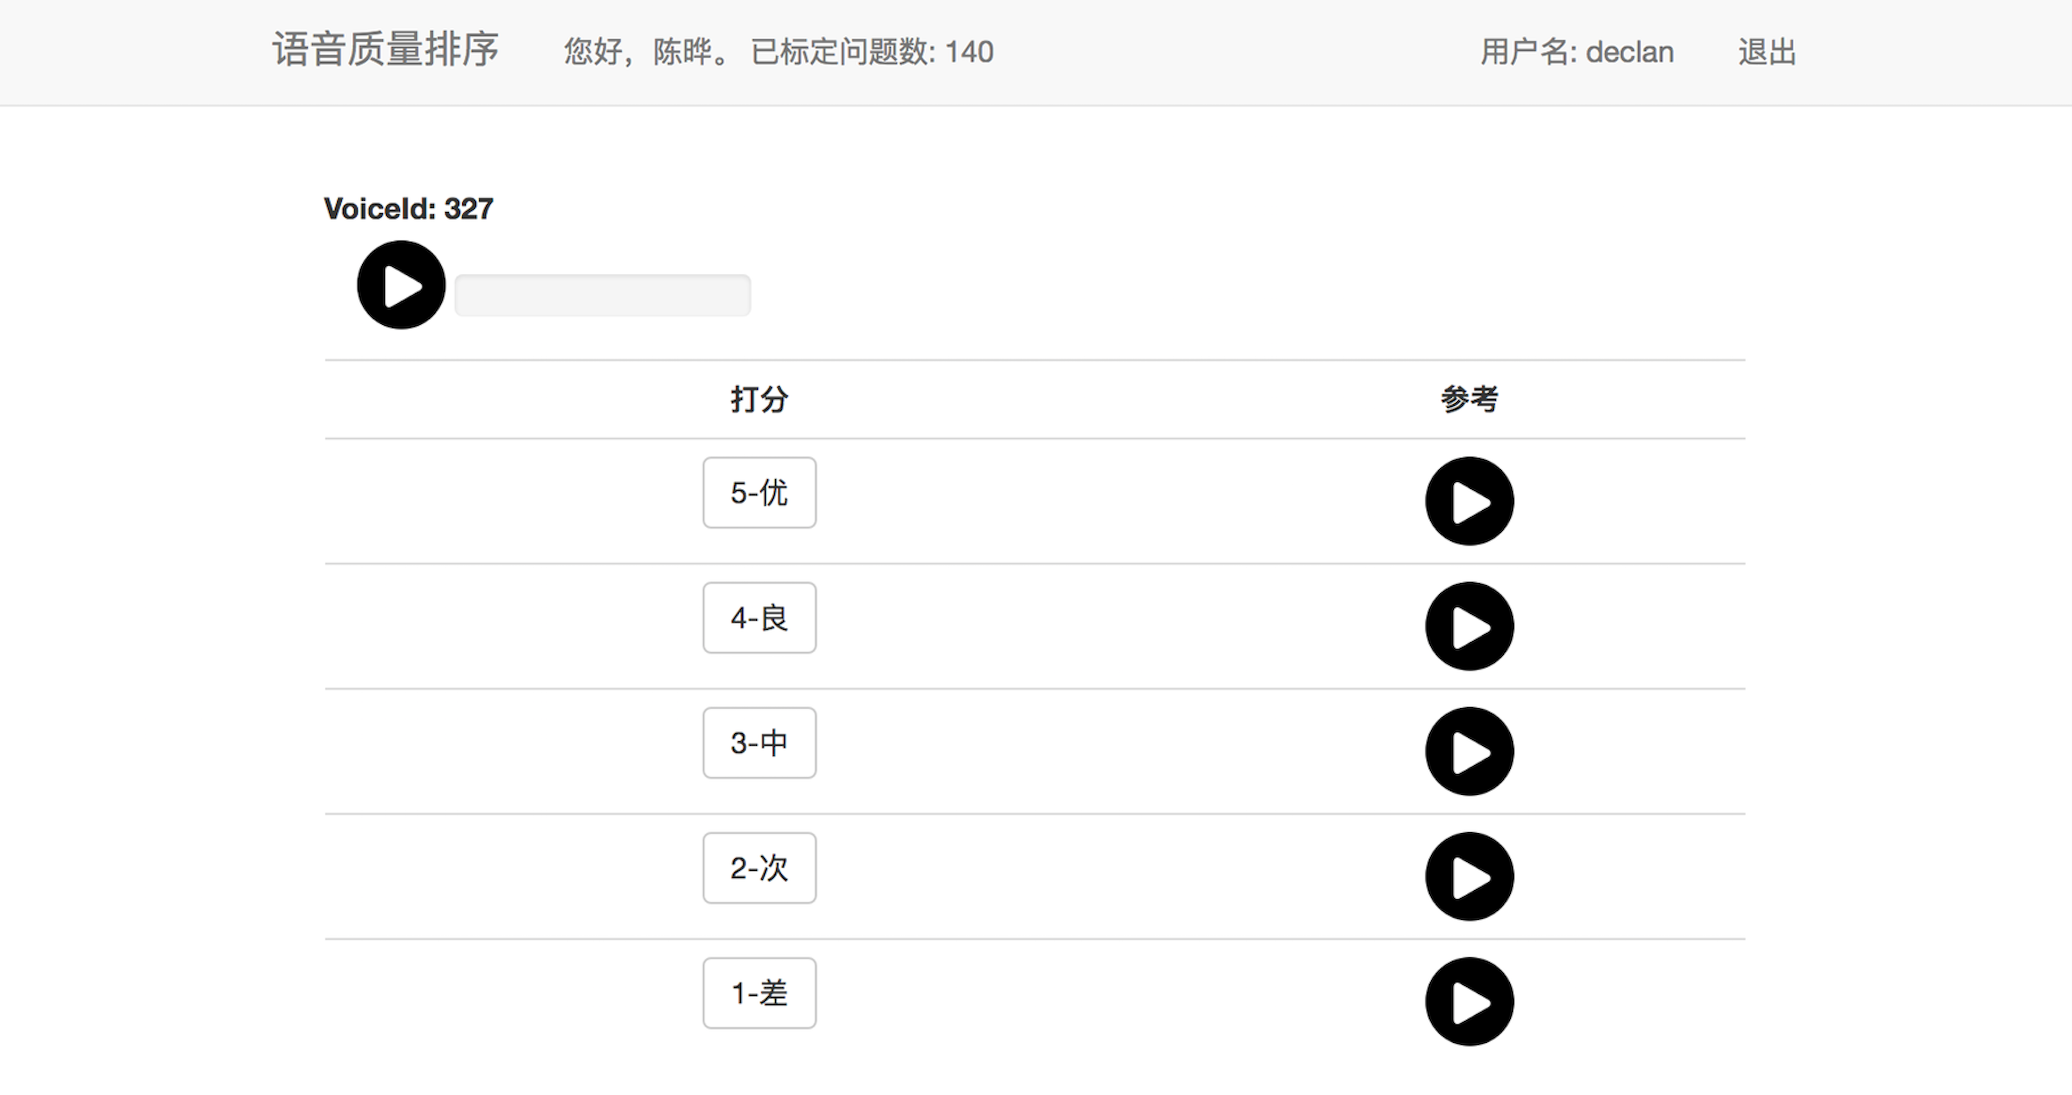
\includegraphics[width=0.45\textwidth]{web-user-mos}
}
\caption{在线辅助系统的志愿者界面\label{fig:web-user}}
\end{figure}

志愿者端则是会显示当前需要完成的主观评分或者比较的问题,供志愿者回答,如图~\ref{fig:web-user}所示,志愿者界面上方显示了志愿者的姓名,已经标定的问题数量等信息。在排序任务中,志愿者的界面如图~\ref{fig:web-user-sort}所示,系统会让志愿者试听两个短波语音,让志愿者选择哪一个质量更优,或者选择两者质量差不多。而在MOS分任务中,志愿者的界面如图~\ref{fig:web-user-mos}所示,系统会给出一个待评分的语音,志愿者对其进行质量评分,选择1~5中的一个分数。每个分数右侧会有预先分组好的各等级语音的参考标准,供志愿者试听比较从而更好的进行评判。志愿者每回答完一个问题,会显示新的问题,直至当前实验中的任务均已完成为止。

\section{系统实现介绍}

短波语音主观评价在线辅助系统实现在Ubuntu 14.04操作系统上,基本环境要求如下:
\begin{itemize}
    \item 操作系统:Ubunutu 14.04
    \item Web服务器: Jetty9.2.24
    \item Java: JRE 7
    \item 数据库:MySQL 5.5
\end{itemize}

系统后端使用Java的Spring框架和Jersey框架实现符合Restful设计理念的API接口,前端使用AngularJs实现单页web应用,符合MVC设计模型,将系统的数据层、逻辑层和表示层完全剥离解耦\cite{burbeck87}。数据库部分使用MySQL数据库存储,包括账户信息数据表、语音队列数据表、语音数据表、语音比较问题表、语音主观评分表,分别如表~\ref{tab:user}\~~\ref{tab:score}所示。

\begin{table}
\centering
\caption{账户信息数据表vs\_user}
\label{tab:user}
\begin{tabular}{ccc}
\toprule[1.5pt]
字段名 & 字段类型 & 备注 \\ \midrule[1pt]
u\_id & bigint(20) & Unsigned, Primary key, Auto Increment \\
u\_username & varchar(255) & 用户名 \\
u\_password & varchar(128) & 加密存储的密码 \\
u\_name & varchar(255) & 真实姓名 \\
u\_role & tinyint(3) & 0: 志愿者,1:管理员 \\
u\_answer\_cnt & int(10) & 回答问题数量 \\
u\_createtime & timestamp & 默认current\_timestamp \\ \bottomrule[1.5pt]
\end{tabular}
\end{table}

\begin{table}
\centering
\caption{语音队列数据表vs\_queue}
\label{tab:queue}
\begin{tabular}{ccc}
\toprule[1.5pt]
字段名 & 字段类型 & 备注 \\ \midrule[1pt]
q\_id & bigint(20) & Unsigned, Primary key, Auto Increment \\
q\_name & varchar(255) & 语音队列的名称 \\
q\_data\_path & varchar(255) & 语音文件的存储目录 \\
q\_length & int(10) & 队列长度(包含语音数量) \\
q\_type & tinyint(4) & 队列类型,0: 排序类型,1: MOS分类型 \\
q\_sorted & tinyint(1) & 排序是否已完成,仅对排序类型有效 \\
q\_active & tinyint(1) & 是否当前激活队列 \\
q\_createtime & timestamp & 默认current\_timestamp \\ \bottomrule[1.5pt]
\end{tabular}
\end{table}

\begin{table}
\centering
\caption{语音数据表vs\_voice}
\label{tab:voice}
\begin{tabular}{ccc}
\toprule[1.5pt]
字段名 & 字段类型 & 备注 \\ \midrule[1pt]
v\_id & bigint(20) & Unsigned, Primary key, Auto Increment \\
v\_queue\_id & bigint(20) & 所属队列的id,对应vs\_queue表中的q\_id字段 \\
v\_path & varchar(255) & 语音文件的存储路径 \\
v\_order & bigint(20) & 当前在队列中所处排序位置 \\
v\_fixed & tinyint(1) & 当前排序位置是否已固定 \\
\end{tabular}
\end{table}

\begin{table}
\centering
\caption{语音比较问题表vs\_compare}
\label{tab:compare}
\begin{tabular}{ccc}
\toprule[1.5pt]
字段名 & 字段类型 & 备注 \\ \midrule[1pt]
c\_id & bigint(20) & Unsigned, Primary key, Auto Increment \\
c\_queue\_id & bigint(20) & 所属队列的id,对应vs\_queue表中的q\_id字段 \\
c\_vid1 & bigint(20) & 待比较语音1的id,对应vs\_voice表中的v\_id字段 \\
c\_vid2 & bigint(20) & 待比较语音2的id,对应vs\_voice表中的v\_id字段 \\
c\_result & tinyint(4) & 比较结果,0:差不多,1:语音1质量更好,2:语音2质量更好 \\
c\_answer\_uid & bigint(20) & 回答者的id,对应vs\_user表中的u\_id字段 \\
c\_post\_time & timestamp & 该问题最近一次被志愿者获取的时间 \\ \bottomrule[1.5pt]
\end{tabular}
\end{table}

\begin{table}
\centering
\caption{语音主观评分表vs\_score}
\label{tab:score}
\begin{tabular}{ccc}
\toprule[1.5pt]
字段名 & 字段类型 & 备注 \\ \midrule[1pt]
s\_id & bigint(20) & Unsigned, Primary key, Auto Increment \\
s\_userid & bigint(20) & 评分志愿者的id,对应vs\_user表中的u\_id字段 \\
s\_queueid & bigint(20) & 所属队列的id,对应vs\_queue表中的q\_id字段 \\
s\_voiceid & bigint(20) & 评分语音的id,对应vs\_voice表中的v\_id字段 \\
s\_score & int(11) & 评分结果 \\
s\_post\_time & timestamp & 评分时间 \\ \bottomrule[1.5pt]
\end{tabular}
\end{table}

\subsection{语音质量排序的实现}

为了实现对短波语音按照主观感受质量进行排序,我们首先基于快速排序算法的思想设计了模糊版本快速排序算法,然后利用数据库和网站技术交互式地实现了该算法,使算法中的原子比较步骤由志愿者在网页进行,而排序算法由后端程序基于数据库记录的数据进行。

首先简单介绍一下快速排序算法的思想,快速排序是采用分治思想的一种排序算法,时间复杂度为$O(NlogN)$。该算法首先选取待排序元素的第一个或随机的一个作为基准元素,然后通过一次$O(N)$时间复杂度的扫描操作,可以确定该元素按照顺序在队列中的位置,同时保证此时在该元素前的元素均比其小,而在该元素之后的元素均比其大,该元素位置固定不动,将队列分成了前后两半,只有递归地对前后两半分别进行此扫描操作,直至所有元素均确定了位置,则排序完成。

\begin{algorithm}
    \caption{模糊快排中的扫描算法}
    \label{alg:fuzzy-sort}
\begin{algorithmic}[1]
\INPUT
    \Statex 待排序队列x[];
    \Statex 待排序区间$[l, r]$;
\OUTPUT
    \Statex 将x[]在$[l, r]$区间内分成$[l, i], [i+1,  j-1], [j, r]$三个区间
    \Statex $[i+1,  j-1]$中的元素均模糊相等
    \Statex $[l, i]$中的元素比上述元素小,$[l, i]$中的元素比上述元素大
\State 基准元素$y = x[l]$
\State $i=l-1, j=r+1, k=l$
\While { $k<j$ 且 $k\leq r$}
    \If { $x[k]<y$; }
        \State 交换$x[i+1], x[k]$的值
        \State $i = i + 1, k = k + 1$
    \ElsIf { $x[k] > y$; }
        \State 交换$x[j-1], x[k]$的值
        \State $j=j-1$
    \Else
        \State (x[k]和y模糊相等) $k=k+1$ 
    \EndIf
\EndWhile
\end{algorithmic}
\end{algorithm}

在语音的主观质量排序中,经常会出现两个语音质量近似相等,难以区分哪一个更优的情况,本文针对此优化设计了模糊版本的快速排序算法,此算法与快速排序算法的很接近,唯一的修改是在每次扫描时,将待排序的区间$[l, r]$划分成$[l, i], [i+1,  j-1], [j, r]$三个区间,其中$[l, r]$中的元素均是比基准元素小的,$[j, r]$中的均是比基准元素大的,而$[i+1,  j-1]$中是与基准元素模糊相等的。之后递归的对左区间和右区间进行扫描即可完成排序。改进的扫描算法的具体实现如算法~\ref{alg:fuzzy-sort}所示。

\begin{figure}
\centering
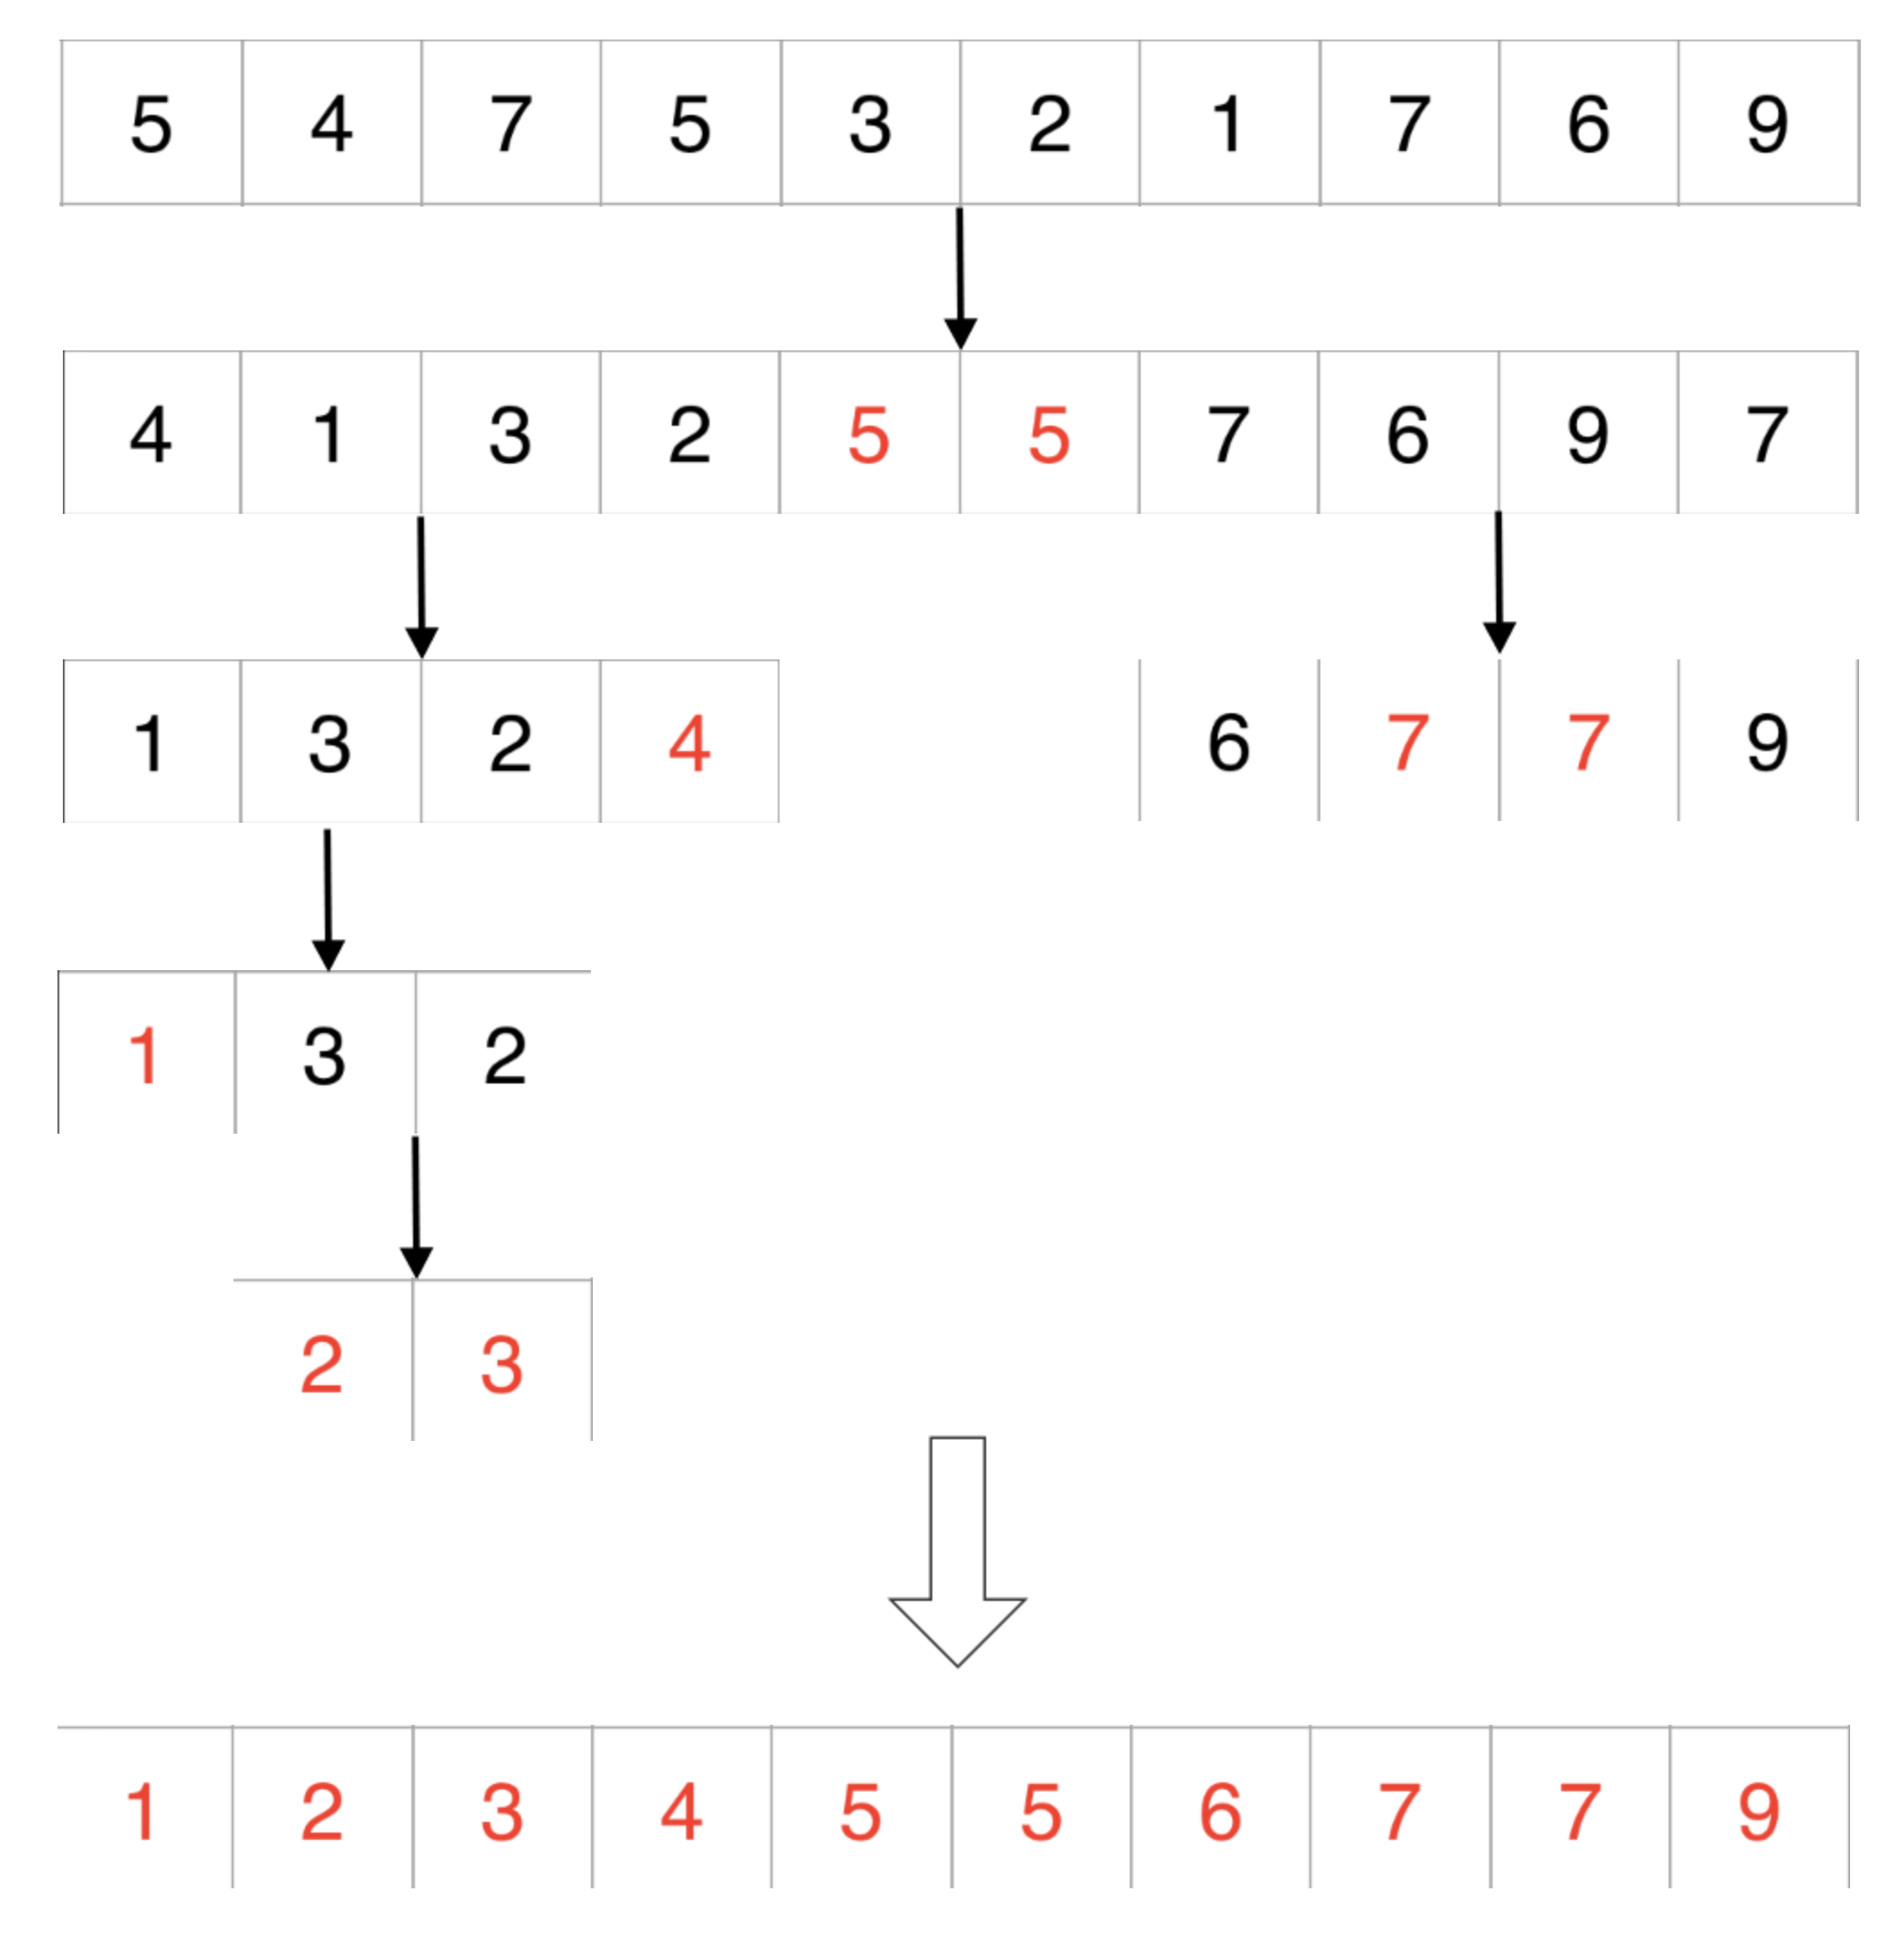
\includegraphics[width=0.8\textwidth]{sort-alg}
\caption{模糊快排算法执行示例\label{fig:fuzzy-sort}}
\end{figure}

图~\ref{fig:fuzzy-sort}演示了模糊快排算法对一列整数进行排序的过程,红色数字表示位置已经确定的数字。由于算法是递归执行,所以执行过程行成了一个树状结构。

\begin{algorithm}
    \caption{交互式模糊快排算法}
    \label{alg:interactive-sort}
\begin{algorithmic}[1]
\INPUT
    \Statex 待排序语音v[],总个数L
\OUTPUT
    \Statex 排序结果order[],对应每个语音的排序位置
\State 初始化order[]为1至L
\State fixed[]数组表示每个语音位置是否已固定,全部初始化为false
\While { $ \exists i, s.t. fixed[i] = false $; }
    \State 将order[]和fixed[]信息存储进vs\_voice表
    \State 根据当前排序状态,参考算法~\ref{alg:fuzzy-sort}生成所有需要比较的语音对,插入vs\_compare表
    \State 等待志愿者回答所有的语音质量比较问题
    \State 根据志愿者的回答,参考算法~\ref{alg:fuzzy-sort}更新所有待定区间的排序状态,更新order[]和fixed[]
\EndWhile
\end{algorithmic}
\end{algorithm}

将该算法应用到短波语音的主观质量排序中时,两个语音的质量比较过程需要由志愿者而非程序完成。所以我们设计了一个基于数据库存储和网站技术的交互式模糊快排算法。主要思想是将排序的递归树按层分,每一层的排序状态可以保存在数据库中。基于排序状态生成当前所有需要进行比较的语音对,将这些比较分发给志愿者回答。当所有问题均已被回答,程序从数据库中读取当前排序状态,根据回答的问题可以排序队列进入到下一层状态中。如此循环往复直至所有语音均排序完毕。具体的存储情况如下:vs\_voice表(参见表~\ref{tab:voice})中存储了每个语音在排序中的位置(v\_order字段),以及位置是否已经固定(v\_fixed字段),这两个信息即可保存队列排序的状态信息;而需要比较的语音对存储在vs\_compare表(参见表~\ref{tab:compare})中,志愿者回答的信息也会保存到该表中。具体算法流程如算法~\ref{alg:interactive-sort}所示。

上述算法中生成的语音比较问题会插入vs\_compare表,下面说明前端获取比较问题给志愿者回答的策略。我们希望尽量减少志愿者重复回答同一问题,所以首先获取没有被其他志愿者获取过的问题。而当目前所有问题均已被获取过,则获取最早分发给志愿者而依然没有被回答的问题。具体实现上在vs\_compare表中有c\_post\_time标记了该比较问题上一次被获取的时间,若还未被获取则为空(null),而c\_answer\_uid记录了回答该问题的志愿者id,如果还未被回答则为空(null)。我们根据这两个字段来获取当前该分发给志愿者的问题。

\subsection{语音MOS分评价的实现}

统计语音的平均主观意见分(MOS)的功能要相对简单一些,建立语音队列时,扫描目录下的语音文件,在vs\_voice中插入所有语音的数据记录。然后每个志愿者可以获取他还没有进行主观评分的语音,在前端展示试听,志愿者根据主观感受进行评分,分值从1-5不等。志愿者主观评分的记录被保存在vs\_score表中,通过统计该表信息,可以得到每条语音数据被几位志愿者评分,以及其平均主观意见分的分值。

\section{小结}

本章介绍了短波语音主观评价在线辅助系统。该系统用于辅助进行短波语音的主观评价工作,包含两种功能:一是通过主观比较对一组短波语音进行质量排序;二是通过记录统计主观评分计算各个短波语音的平均主观意见分。我们首先介绍了系统的功能和使用,然后介绍了系统的实现。